
\documentclass[10pt,landscape]{extarticle}
\usepackage{amssymb,amsmath,amsthm,amsfonts}
\usepackage{multicol,multirow}
\usepackage{calc}
\usepackage{ifthen}
\usepackage[landscape]{geometry}
\usepackage[colorlinks=true,citecolor=blue,linkcolor=blue]{hyperref}
\usepackage{graphicx}
\usepackage{commath}
\usepackage{listings}
\usepackage{microtype}
\usepackage[compact,small]{titlesec}
\usepackage{enumitem}
\setenumerate{noitemsep,topsep=0pt,parsep=0pt,partopsep=0pt}
\setitemize{noitemsep,topsep=0pt,parsep=0pt,partopsep=0pt}
\graphicspath{ {./images/} }
\ifthenelse{\lengthtest { \paperwidth = 11in}}
    { \geometry{top=.5cm,left=.5cm,right=.5cm,bottom=.5cm} }
	{\ifthenelse{ \lengthtest{ \paperwidth = 297mm}}
		{\geometry{top=1cm,left=1cm,right=1cm,bottom=1cm} }
		{\geometry{top=1cm,left=1cm,right=1cm,bottom=1cm} }
	}
\pagestyle{empty}
\makeatletter
\renewcommand{\section}{\@startsection{section}{1}{0mm}%
                                {-1ex plus -.5ex minus -.2ex}%
                                {0.5ex plus .2ex}%x
                                {\normalfont\large\bfseries}}
\renewcommand{\subsection}{\@startsection{subsection}{2}{0mm}%
                                {-1ex plus -.5ex minus -.2ex}%
                                {0.3ex}%
                                {\normalfont\small\bfseries}}
\renewcommand{\subsubsection}{\@startsection{subsection}{2}{0mm}%
                                {-1ex plus -.5ex minus -.2ex}%
                                {0.2ex}%
                                {\normalfont\small\bfseries}}                                
\makeatother
\setcounter{secnumdepth}{0}
\setlength{\parindent}{0pt}
\setlength{\parskip}{0pt plus 0.5ex}
% -----------------------------------------------------------------------

\title{Cheat sheet}

\begin{document}

\raggedright
\footnotesize

\begin{center}
     \Large{\textbf{Computational Structure - Cheatsheet - W3-W5}} \\
\end{center}
\begin{multicols*}{5}
\setlength{\premulticols}{1pt}
\setlength{\postmulticols}{1pt}
\setlength{\multicolsep}{1pt}
\setlength{\columnsep}{2pt}

\section{Week 8}

\subsection{CPU Design Tradeoffs}
\begin{enumerate}
\item Maximum Performance
\item Minimum Cost
\item Best Performance - MIPS = $\frac{Clock Frequency (MHz)}{clocks per instruction}$
\end{enumerate}
Instruction classes - OP,OPC,MEM,Transfer of Control 

\subsection{Multi-Port Register Files}
\begin{enumerate}
\item 2 combinational Read ports
\item 1 clocked Write port - Write Address,Write Data,Write Enable
\end{enumerate}
\subsection{Exception}
Bad Opcode \\ Reg[XP] $\leftarrow$ PC + 4 , PC $\leftarrow$  illOp \\
Other \\ Reg[XP] $\leftarrow$ PC + 4 , PC $\leftarrow$  Xadr \\
\begin{enumerate}
\item Illegal OPCODE in instruction word
\item Reference to non-existent memory
\item Divide by 0
\end{enumerate}
\subsection{Extending Beta}
\subsubsection{LDX(R0,R1,R2)}
ADD(R1,R0,R0) ,
LD(R0,0,R2) \\
Reg[Rc] $\leftarrow$ Mem[ Reg[Ra] + Reg[Rb] ] \\
\subsubsection{STX(R0,R1,R2)}
ADD(R1,R0,R0) ,
ST(R2,0,R0) \\
Mem[ Reg[Ra] + Reg[Rb] ] $\leftarrow$ Reg[Rc] \\
Must amend data path and register file! 
Register file needs another RA/RD port. RA2SEL mux can be removed.

\begin{enumerate}
\item
\end{enumerate}



\section{Week 9}
\section{Memory Hierarchy}
From fastest and most expensive: Cache,SRAM,DRAM, Hard desk \\
Both SRAM and DRAM are volatile storage
\subsection{SRAM}
Static RAM 
\begin{enumerate}
\item 6 transitors and amp sense in each cell with 2 bit line
\item Value stays the same if word line is 0
\item Store a bit
\end{enumerate}
\subsection{DRAM}
\begin{enumerate}
\item 1 transitors and a capacitor
\item A lot cheaper as lesser mosfet used
\item Store a bit
\item Capacitor is leaky, it has to be refreshed frequently, causing it to be significantly slower.
\end{enumerate}
\subsection{Disk}
SSD/HDD \\
Non volatile storage (Can store information even after power source is cut)


\section{The Cache Idea}
\begin{enumerate}
\item Look for requested info in cache
\item If found, it's a hit. Else, go to physical memory and subsequently disk.
\end{enumerate}
\subsection{Locality of references}
Reference to memory location X at time t implies that reference to X + change(X) at
t +change(t) becomes more probable as change(X);change(t) approaches zero.

\section{Type of Cache}
\subsection{Fully Associative Cache(FA)}
Pros: Parallel Lookup and Flexible,address can be stored on any cache line \\
Cons: Needs many Bool operator(1 for each cache line). Also need a replacement strategy. \\ 
\begin{enumerate}
\item TAG contains the all bits of address A
\item DATA contains all bits of content at A: Mem[A]
\item Expensive, made up of SRAMS and other hardwares (comparator circuit
at each row)
\item PARALLEL lookup, hence making it fast
\item Flexible because memory address + content can be stored on any TAG-DATA
row.
\item However, one needs replacement strategy to decide which of the cache line
to write to when cache is full
\end{enumerate}

\subsection{Direct mapping Cache(DM)}
Pros: Cheaper as only 1 Bool operator , No need replacement strategy\\
Cons: Contention - \\
\begin{enumerate}
\item TAG contains T-upper bits of address A
\item DATA contains all bits of content at A: Mem[A]. The lower K-bits of A decides
which ’row’ of DM cache we are looking for. A unique combination of K-bits of
A is mapped to exactly one of the rows of DM cache, hence making it inflexible. 
\item Although it is also made of SRAMS, it is cheaper than FA caches because it is
made up of less hardware (only one comparator circuit per DM cache)
\item No parallelism, but fast mapping between address and cache line
index 
\item Hence, DM cache suffers contention (collision problem) in mapping, two different addresses can be mapped to the same location when the K-lower bits are the same. K-lower bits selected due to locality of reference, but does not completely
eliminate contention.
\end{enumerate}



\subsection{Cache Design Issues}
\begin{itemize}
\item Associativity : how many different address can be stored in the cache
\item Replacement strategy
\item Block size
\item Write strategy
\end{itemize}

\subsection{N-way set associative cache}
\begin{enumerate}
\item if N = 1, it is a DM cache.
\item if k = 1, it is a FA cache
\item Same Column $\implies$ same cache line
\item k lower bits determines the set in which it will be in. 
\end{enumerate}


\subsection{Replacement Strategy}
\begin{enumerate}
\item Least Recently Used: overhead is O(N$\log_{2}{N}$)
\item FIFO: O($log_{2}{N}$) bits/set
\item Random - uses psedu random generator to get reproducible behavior
\end{enumerate}

\subsection{Block Size}
Blocks of $2^{B}$ words per row,

\subsection{Special Bits}
\subsubsection{Valid Bit}
The valid bit indicates that the particular cache row (also called cache line, but it
is a different graphical representation from ’cache line’ in the N-way set associative
cache) contains data from memory and not empty or redundant value. We only
check cache lines with valid bit = 1.
\subsubsection{Dirty Bit}
The dirty bit is set to 1 iff the CPU writes to cache and it hasn’t been stored to the
memory (memory is outdated).
\subsubsection{LRU}
The LRU bit is present in each cache line (for FA), and each cache set-cacheline cell
(for NW), regardless of the block size because R/W with block size more than 1
is always done in parallel.

\section{Cache Writes}
\subsection{Write-through}
CPU writes are done in the cache first by setting TAG = Addr, and Data = new
Mem[Addr] in an available cache line, but also written to the main memory immediately.
This stalls the CPU until write to memory is complete, but memory always
holds the ”truth”
\subsection{Write-behind}
Write to the main memory is buffered or pipelined. CPU keeps executing next instructions while writes are
completed (in order) in the background. 
\subsection{Write-back}
Not immediately written to the main memory. Memory
contents can be ”stale”. Typically CPU will write to the main memory only if the
data in cache line needs to be replaced and that this data has been changed or is
new. This requires the dirty bit in the cache.


\end{multicols*}
\begin{multicols*}{4}


\setlength{\premulticols}{1pt}
\setlength{\postmulticols}{1pt}
\setlength{\multicolsep}{1pt}
\setlength{\columnsep}{2pt}
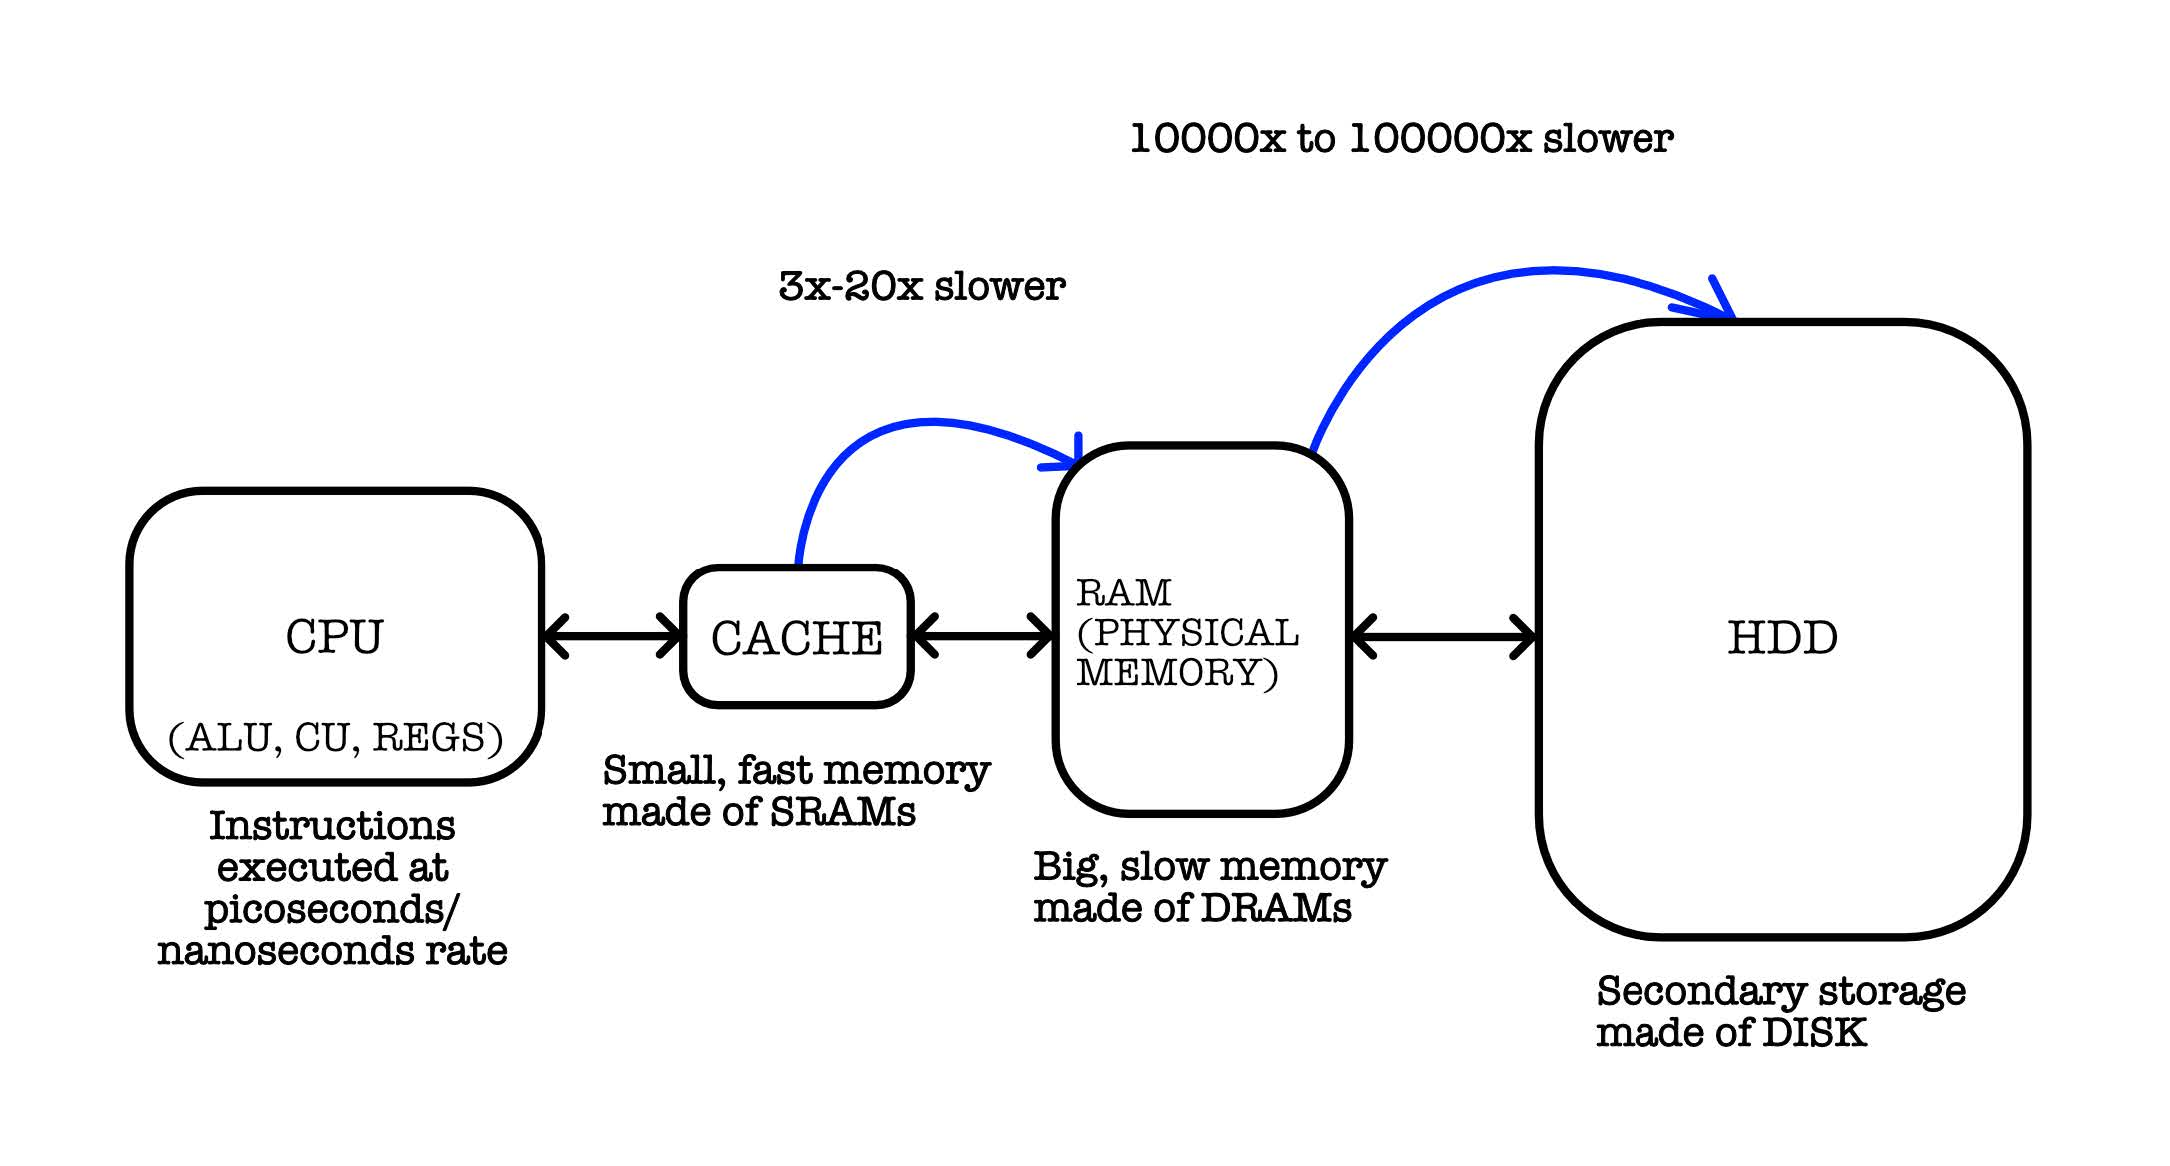
\includegraphics[width = 7cm]{MemoryHierarchy}
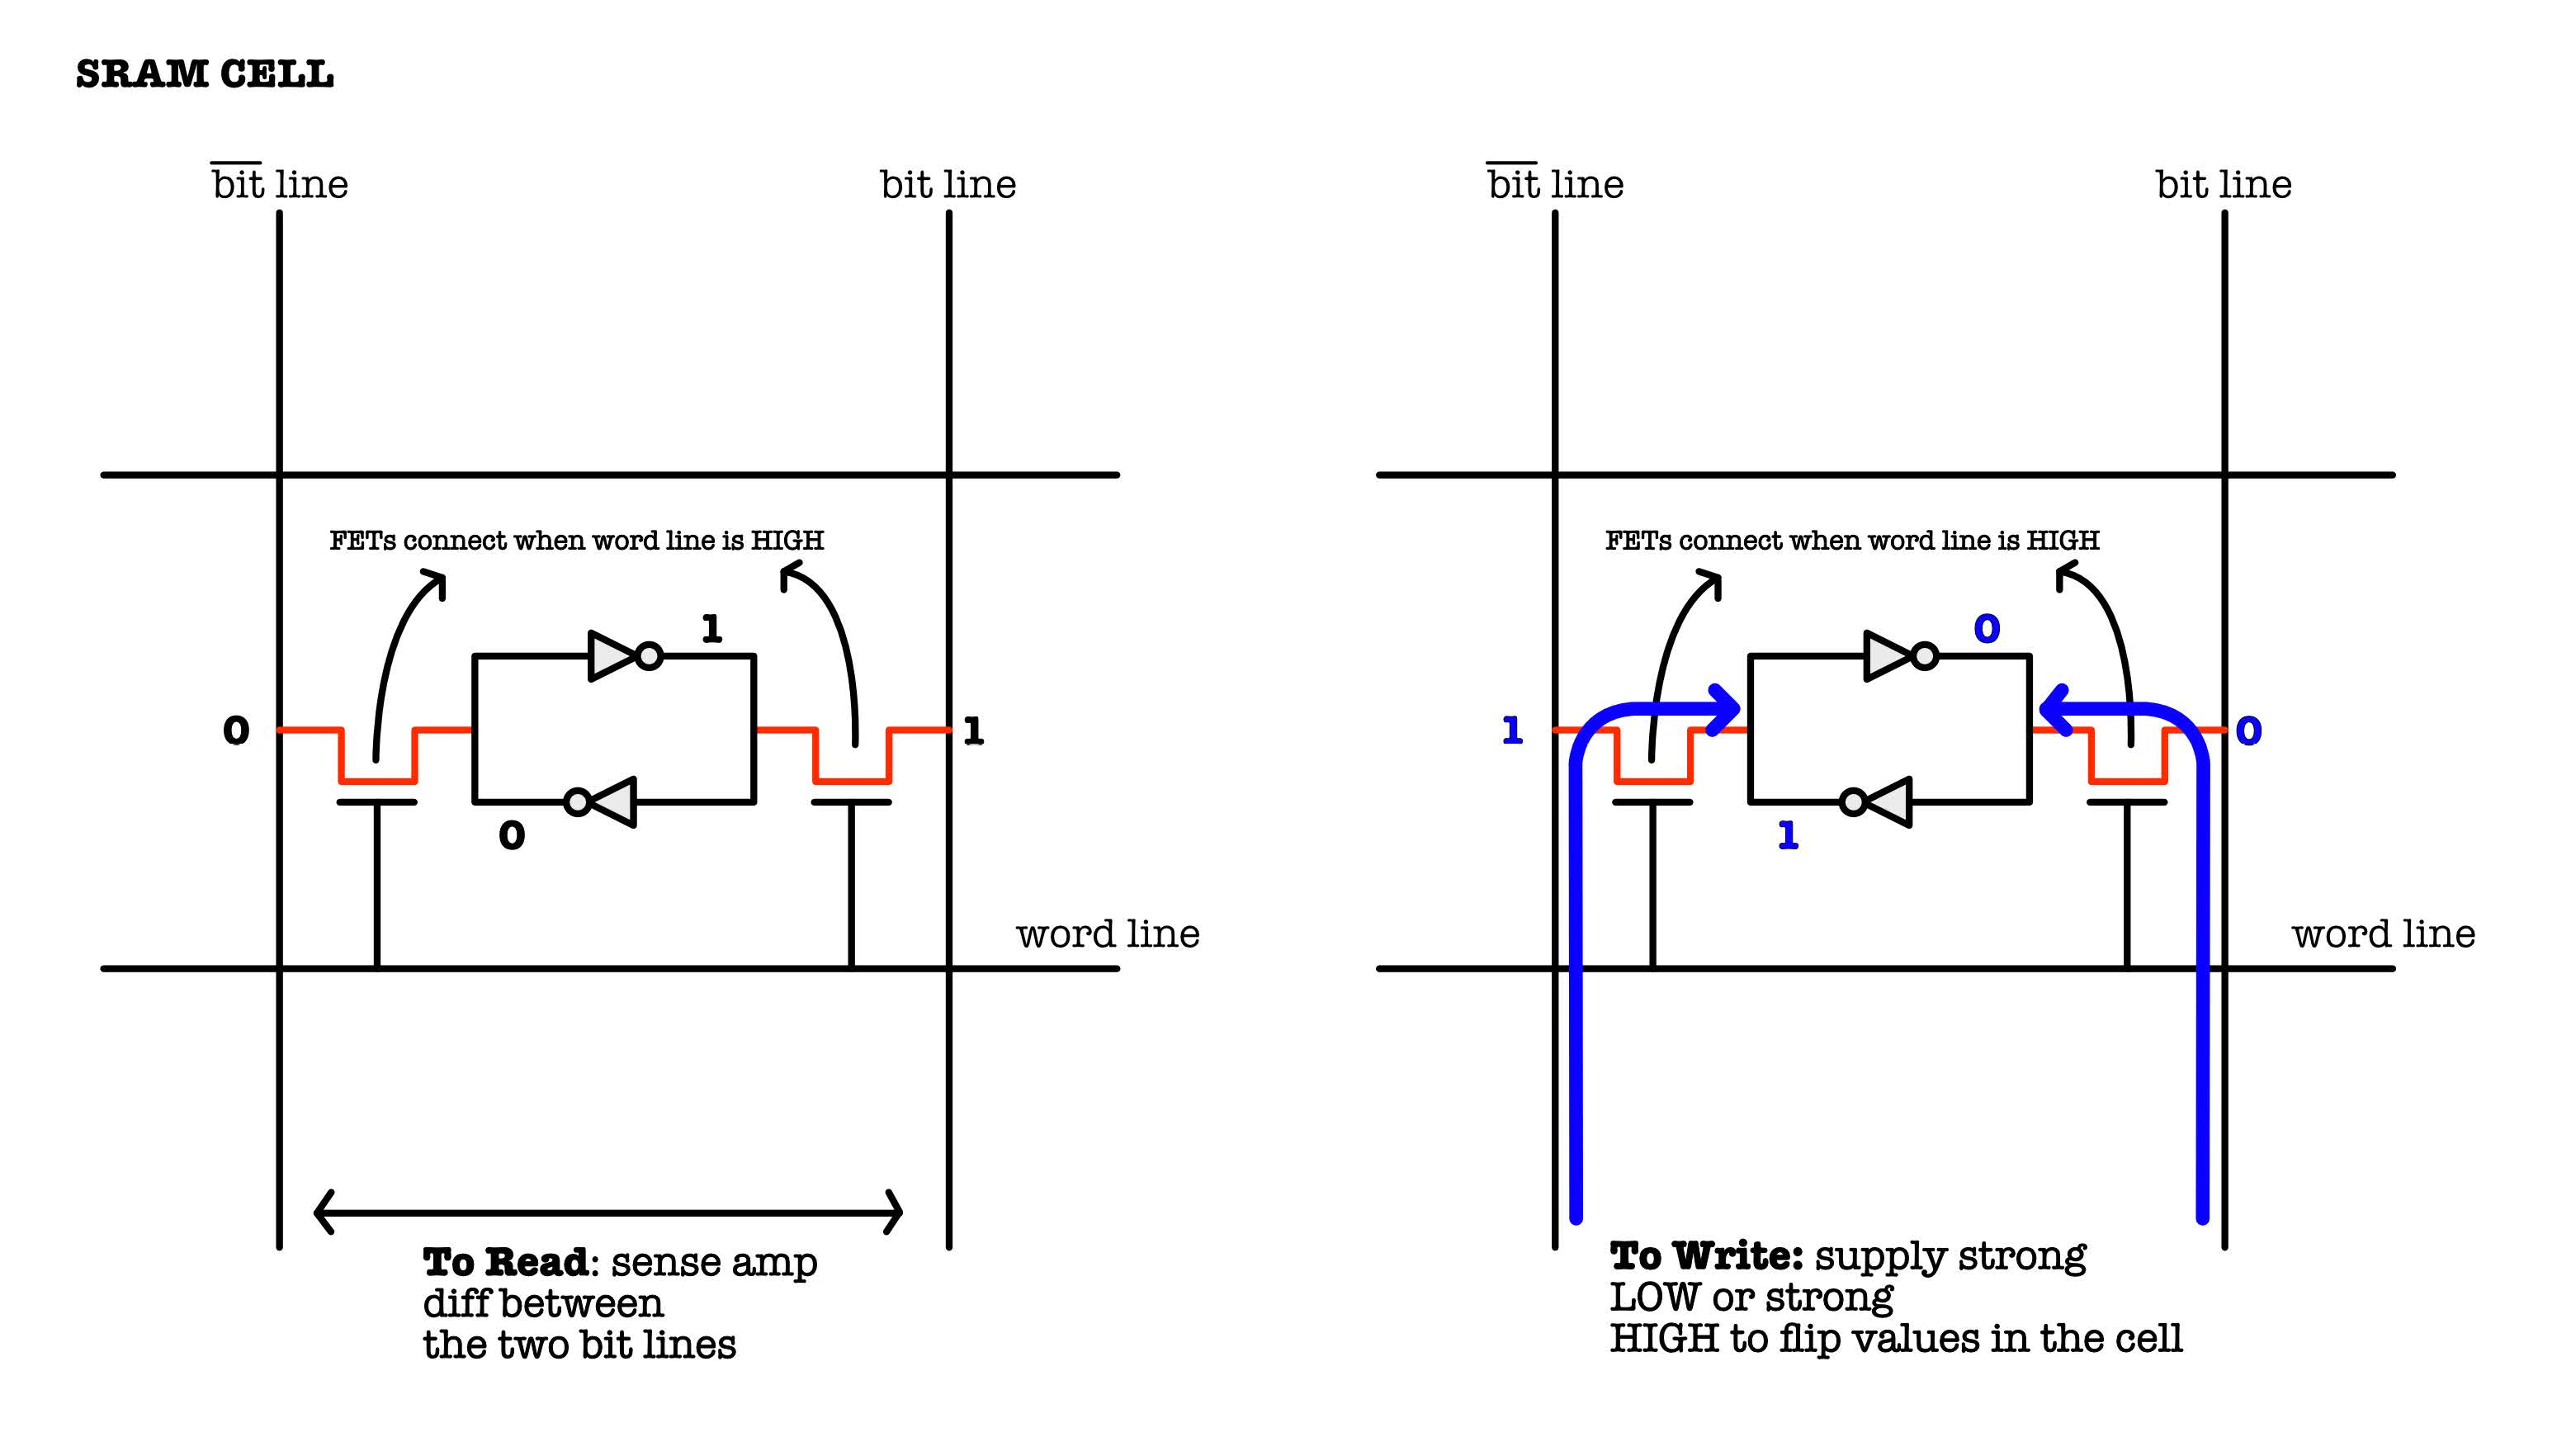
\includegraphics[width = 7cm]{SRAM_cell}
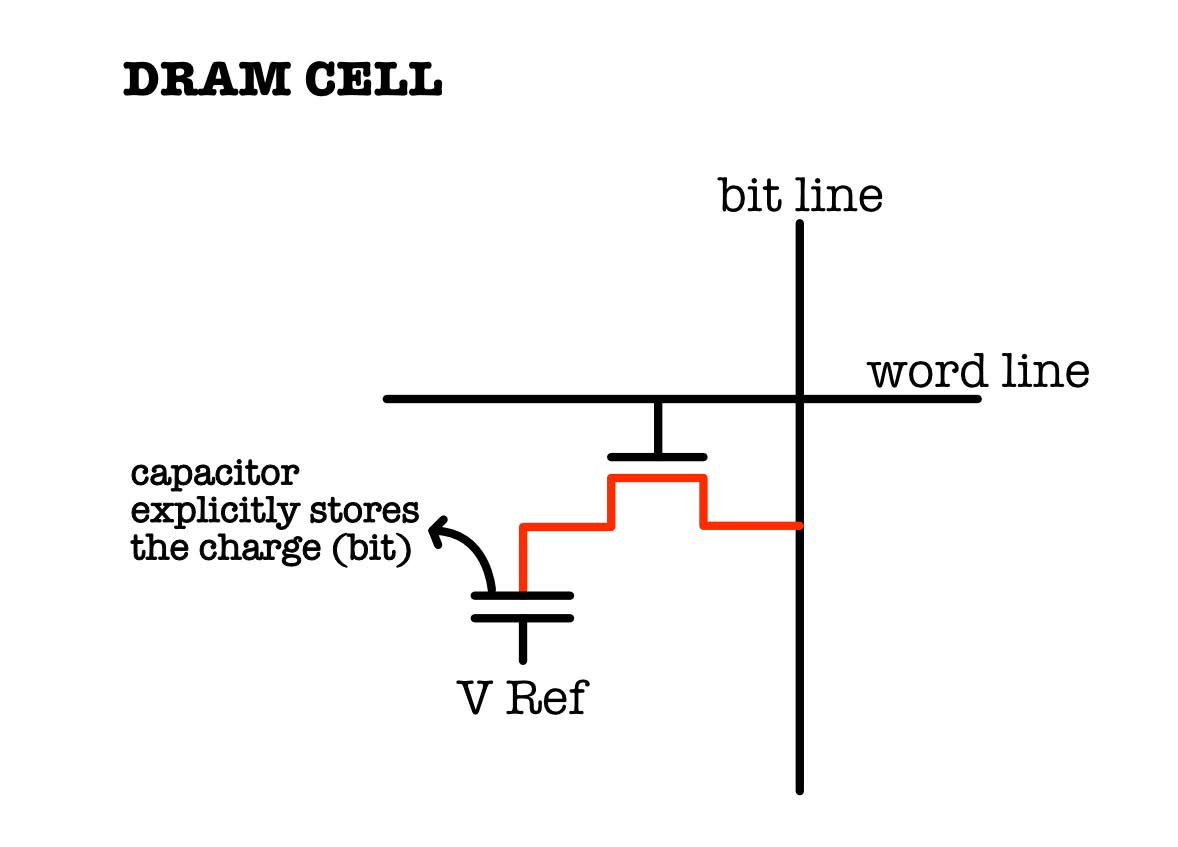
\includegraphics[width = 7cm]{DRAM_cell}
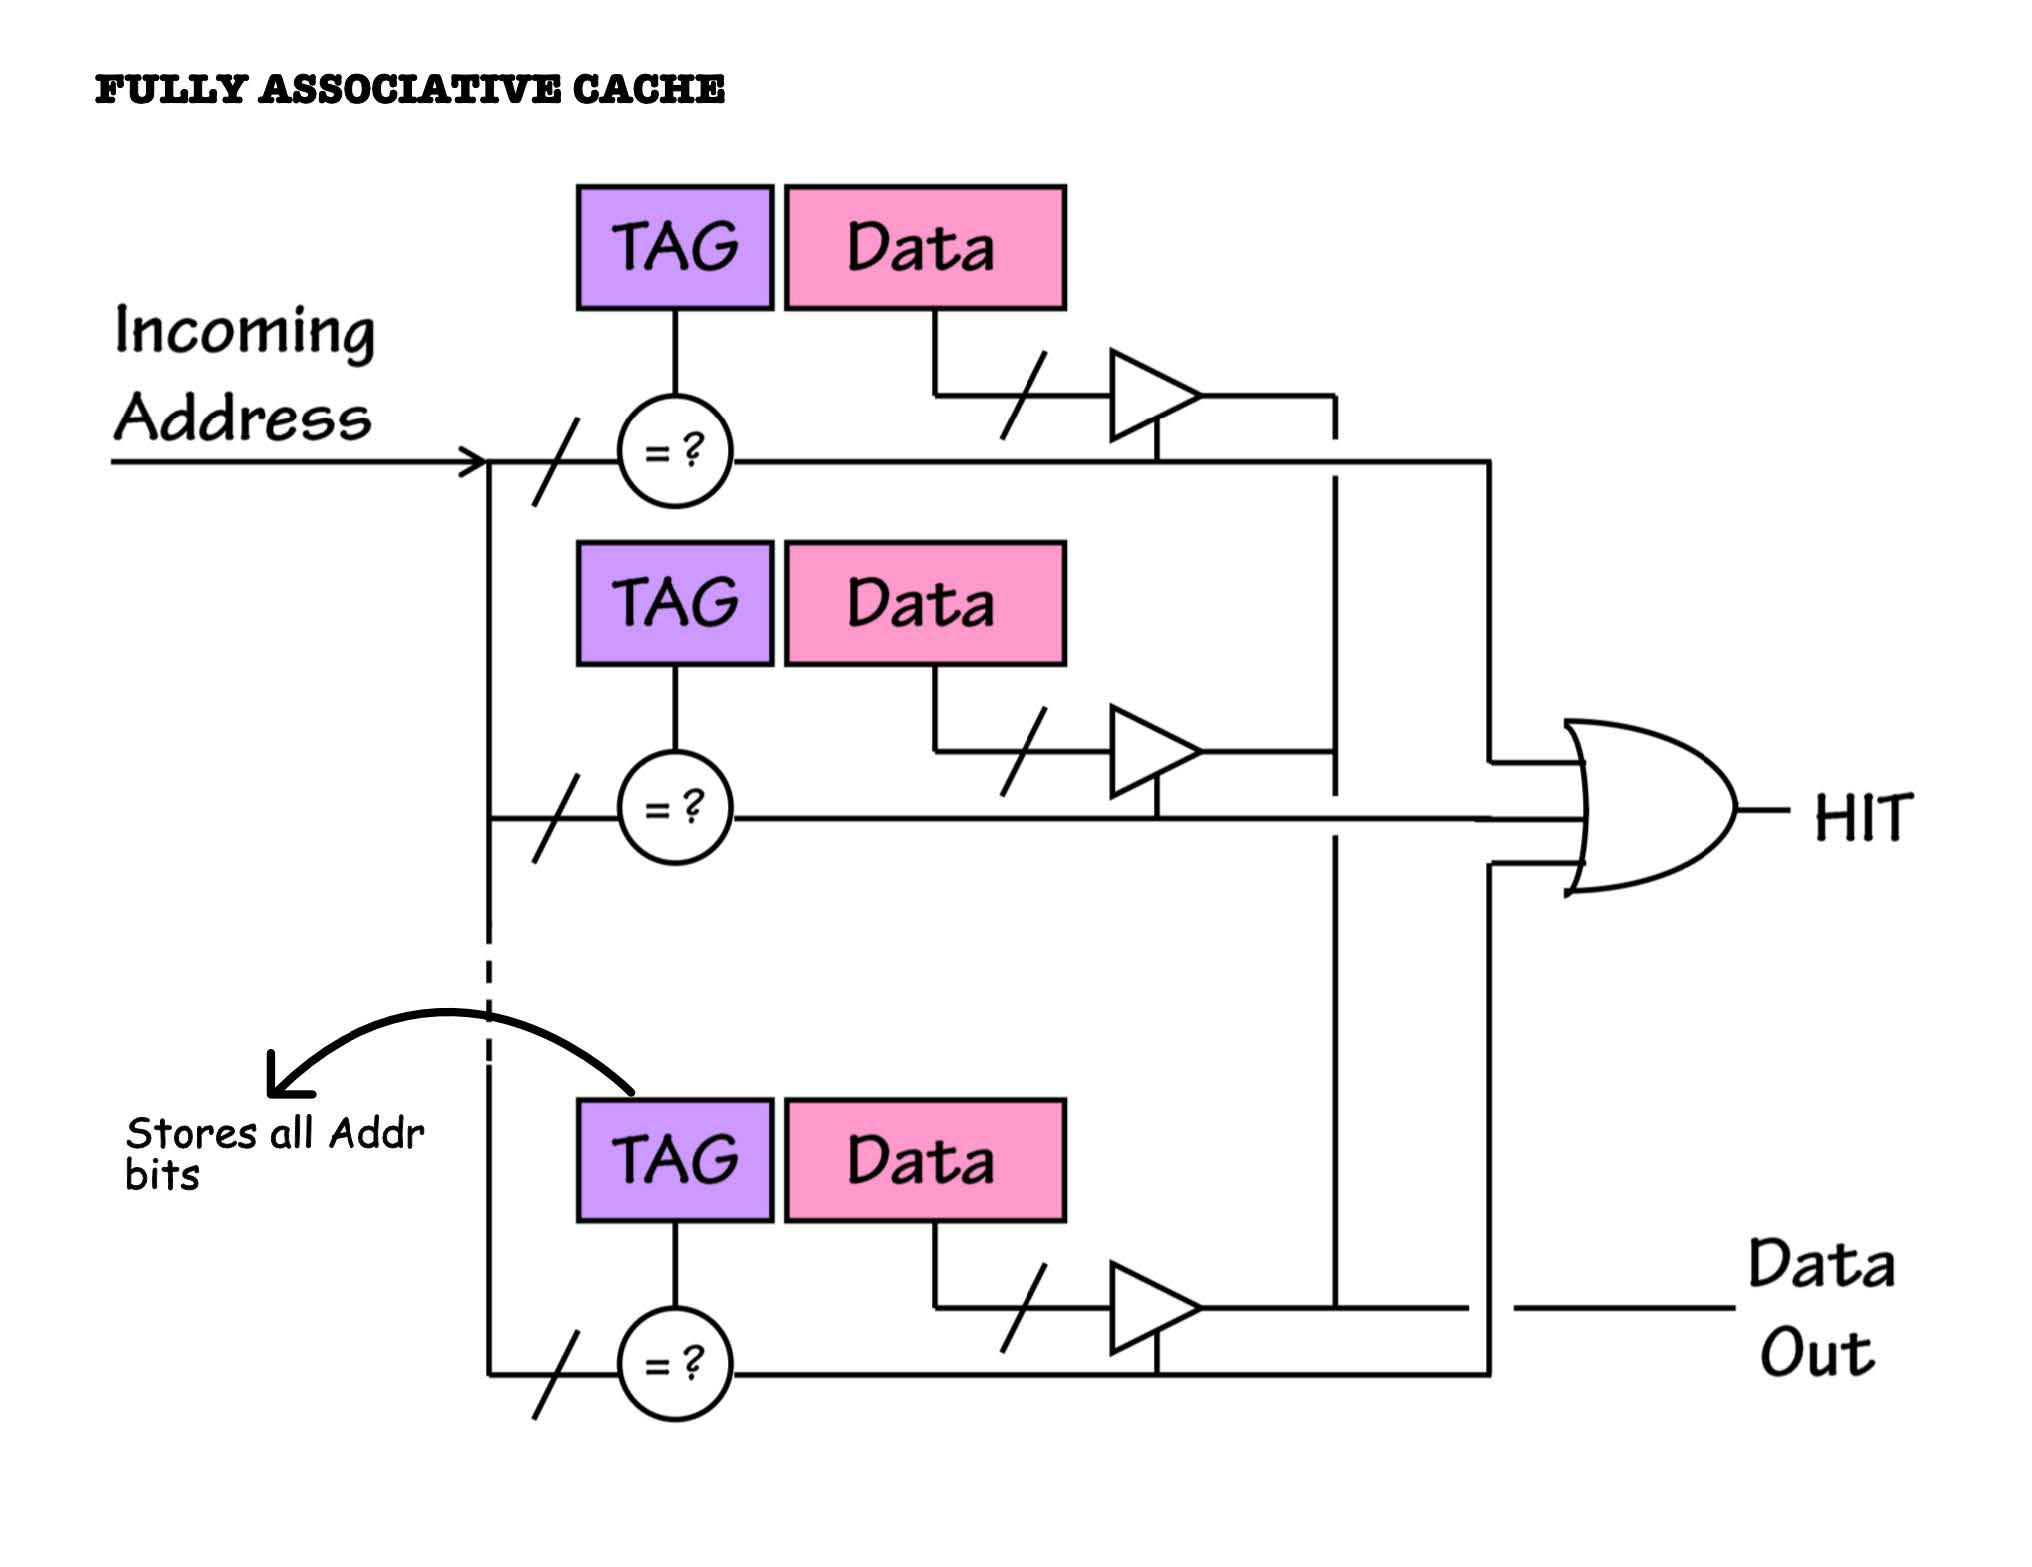
\includegraphics[width = 7cm]{FA_cache}
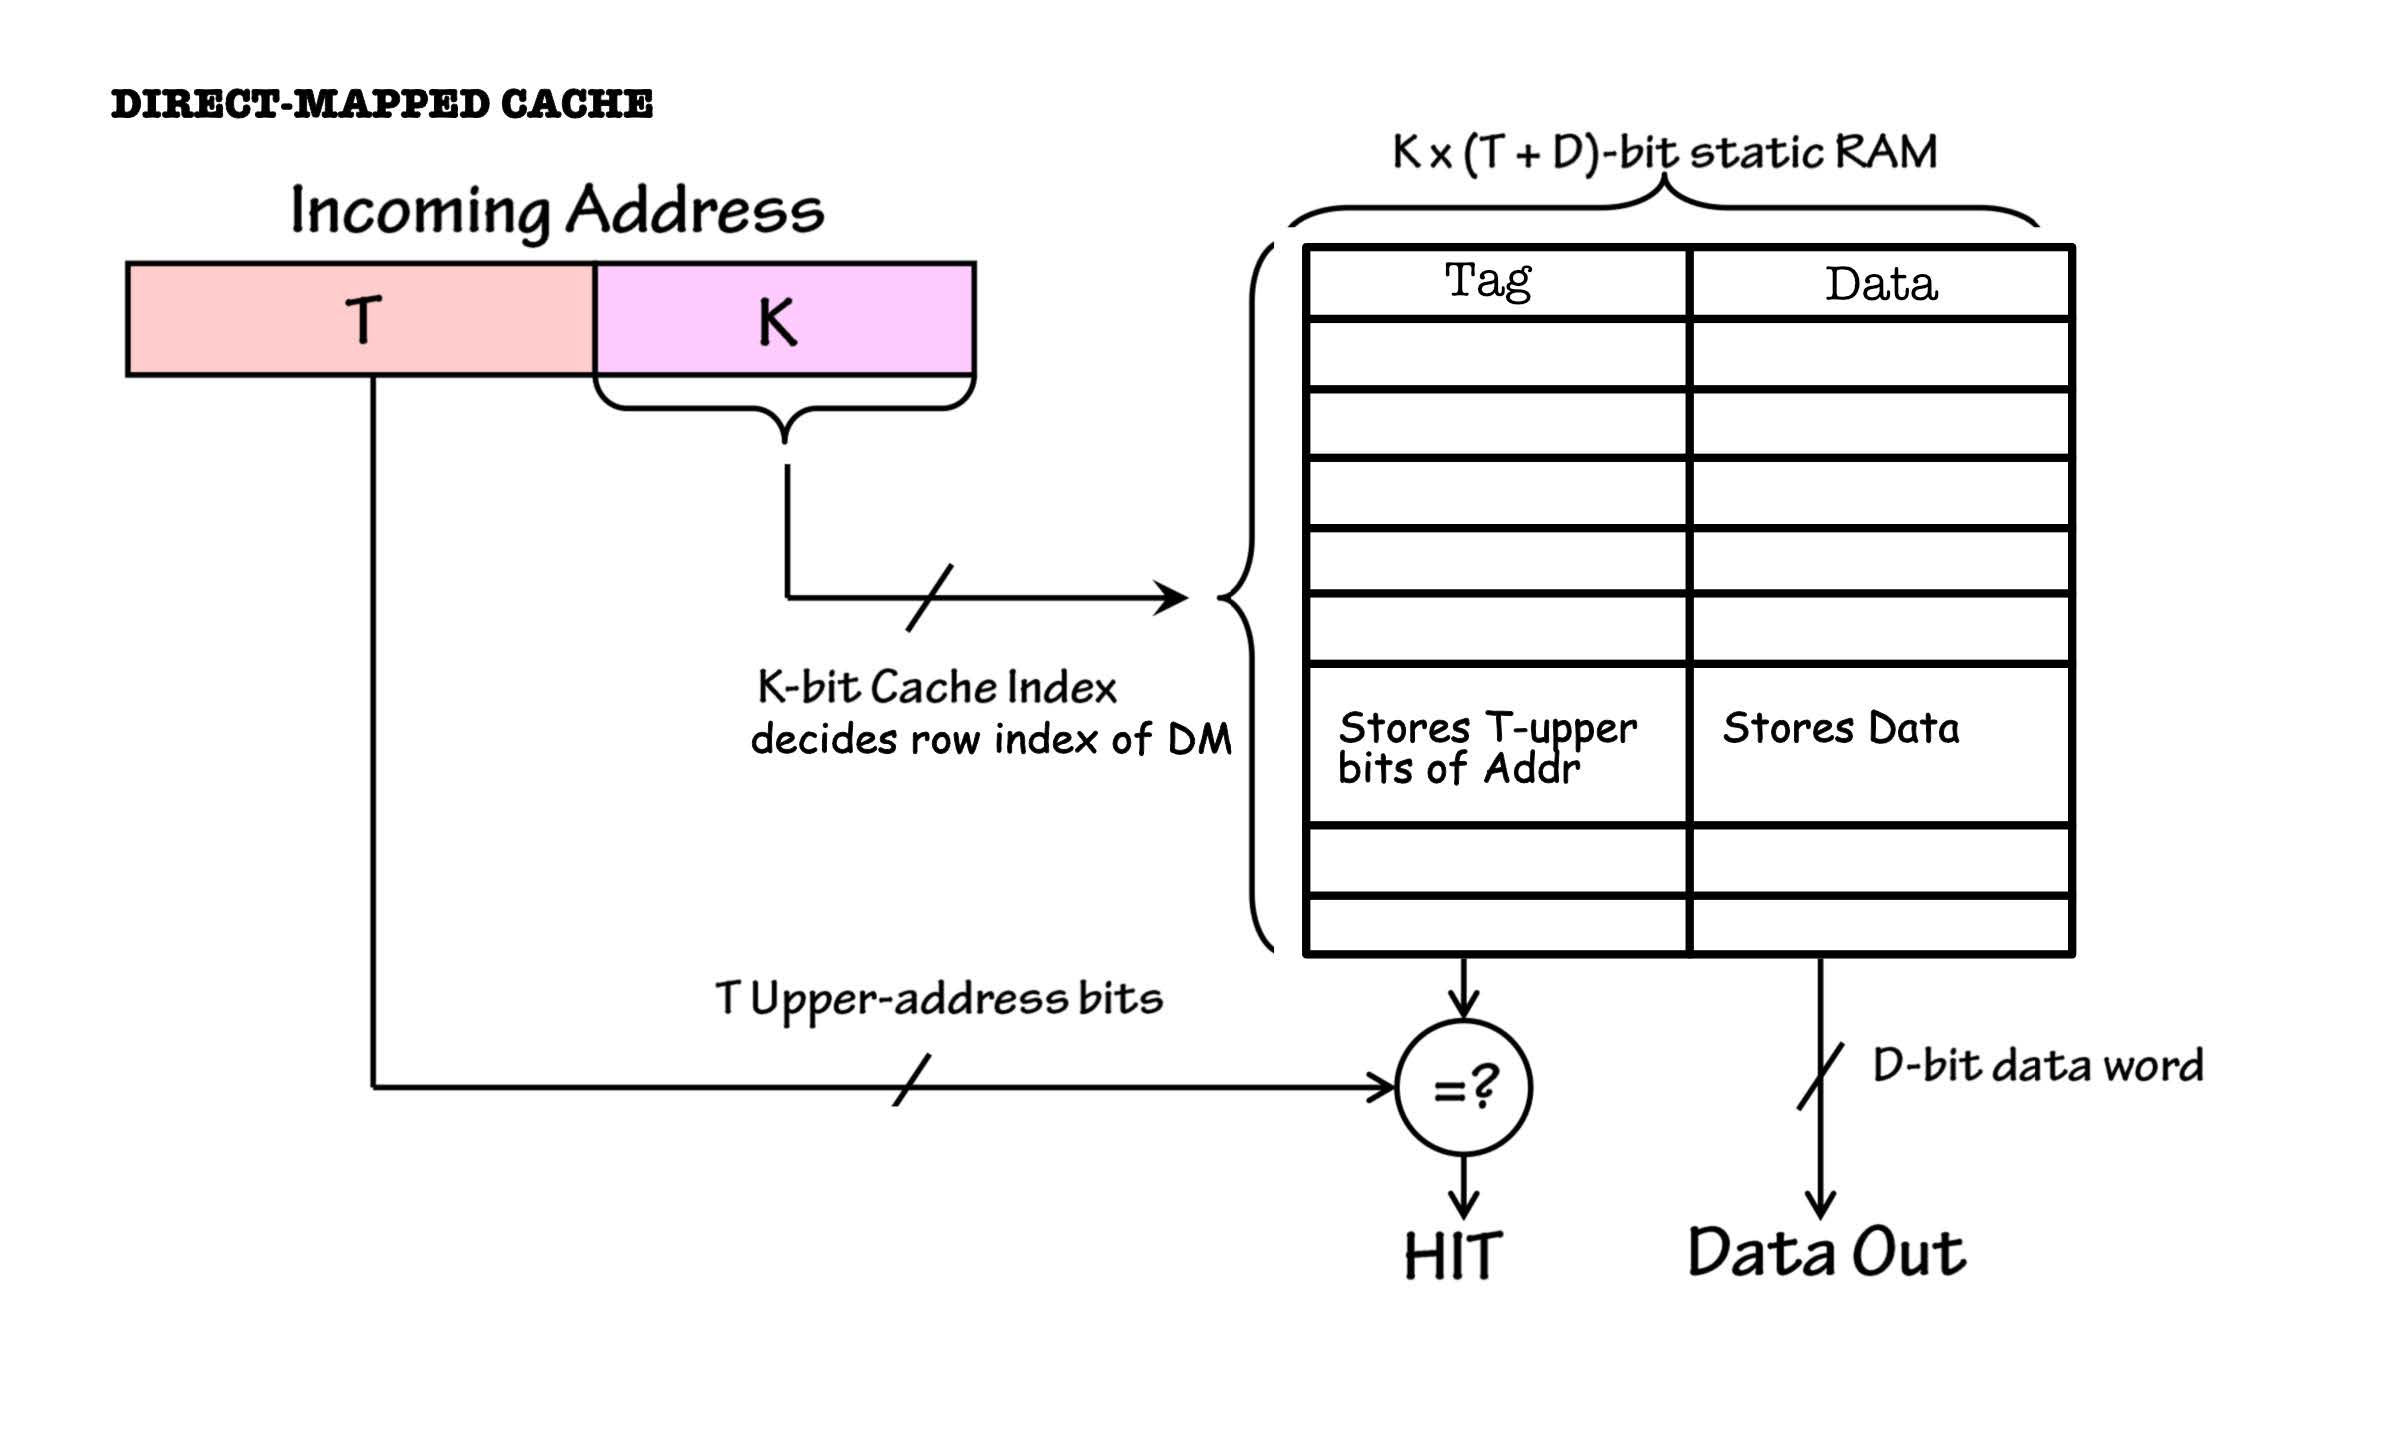
\includegraphics[width = 7cm]{DM_cache}
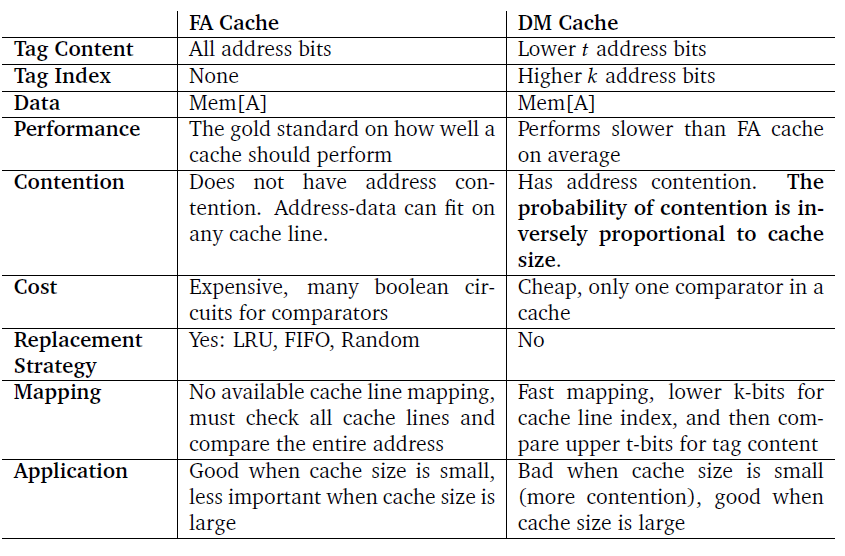
\includegraphics[width = 7cm]{cache_comparison}
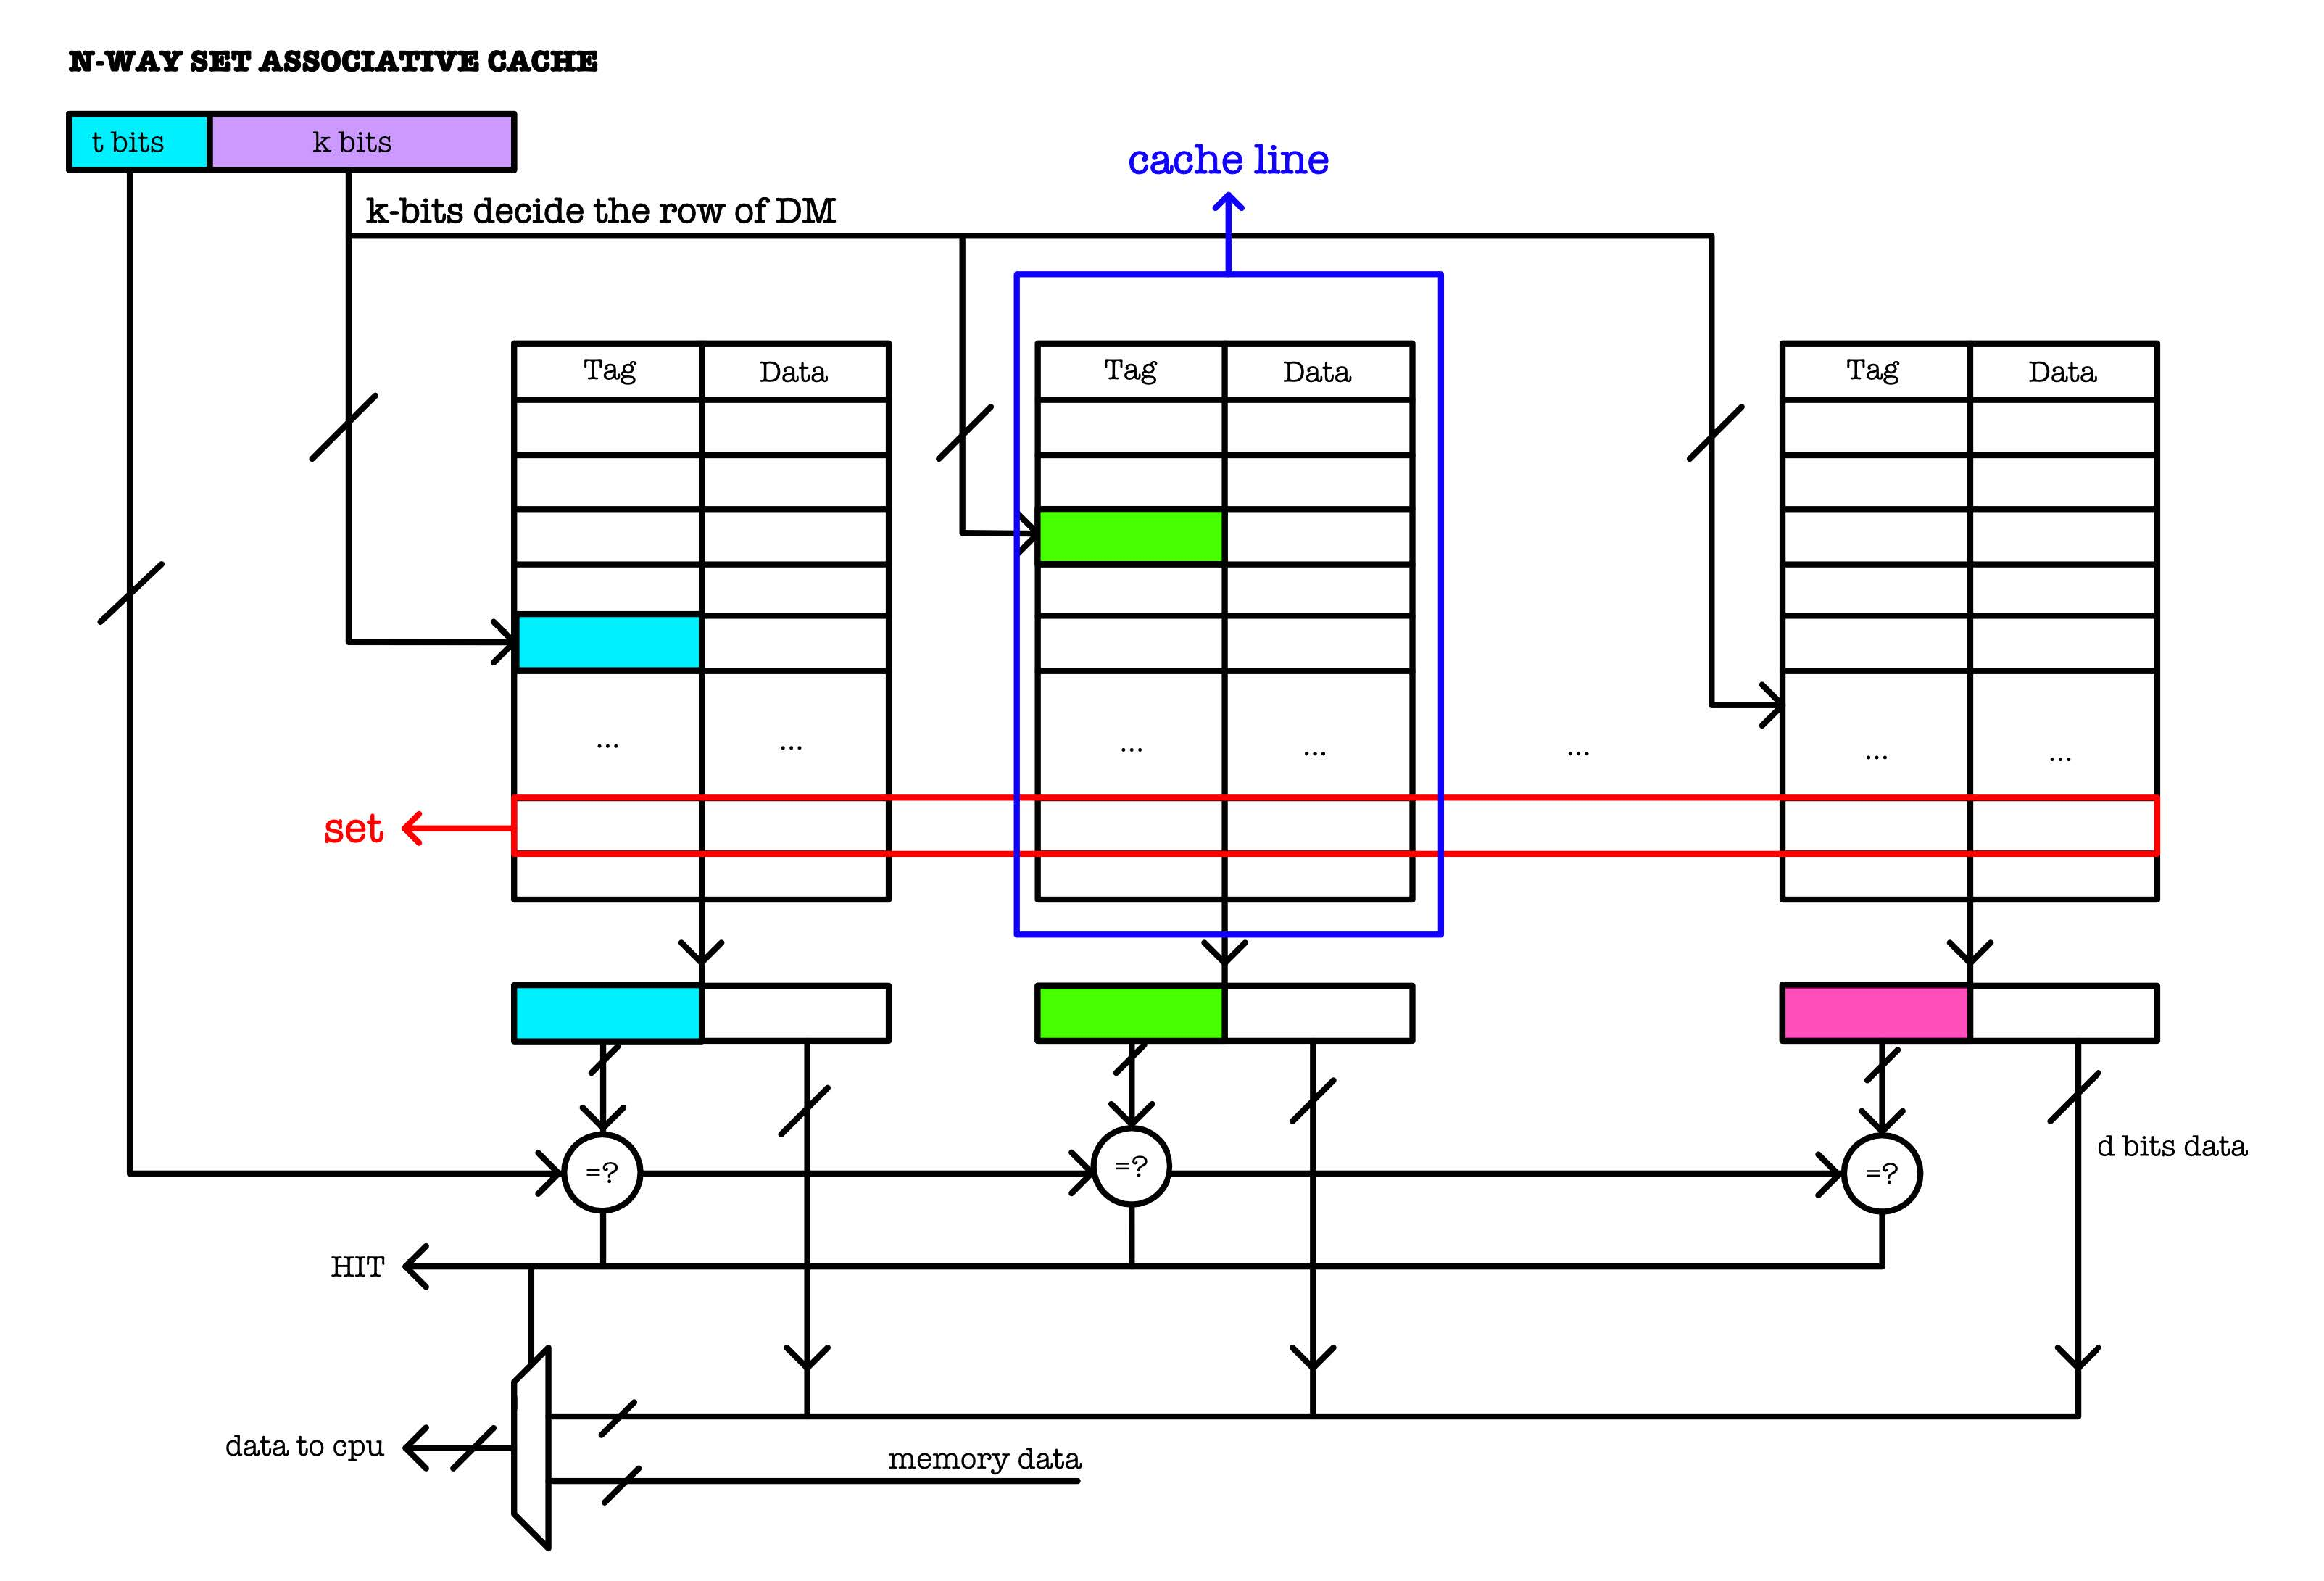
\includegraphics[width = 7cm]{N_way_cache}
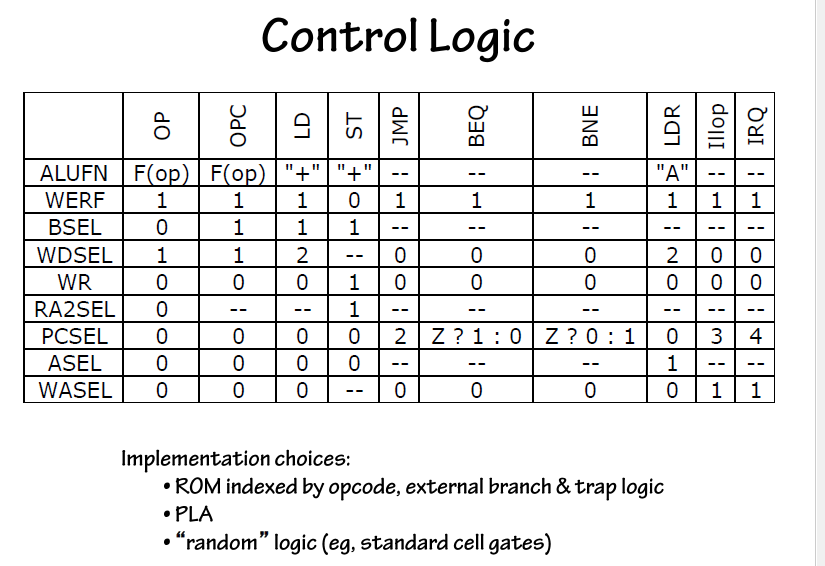
\includegraphics[width = 7cm]{Control_logic}
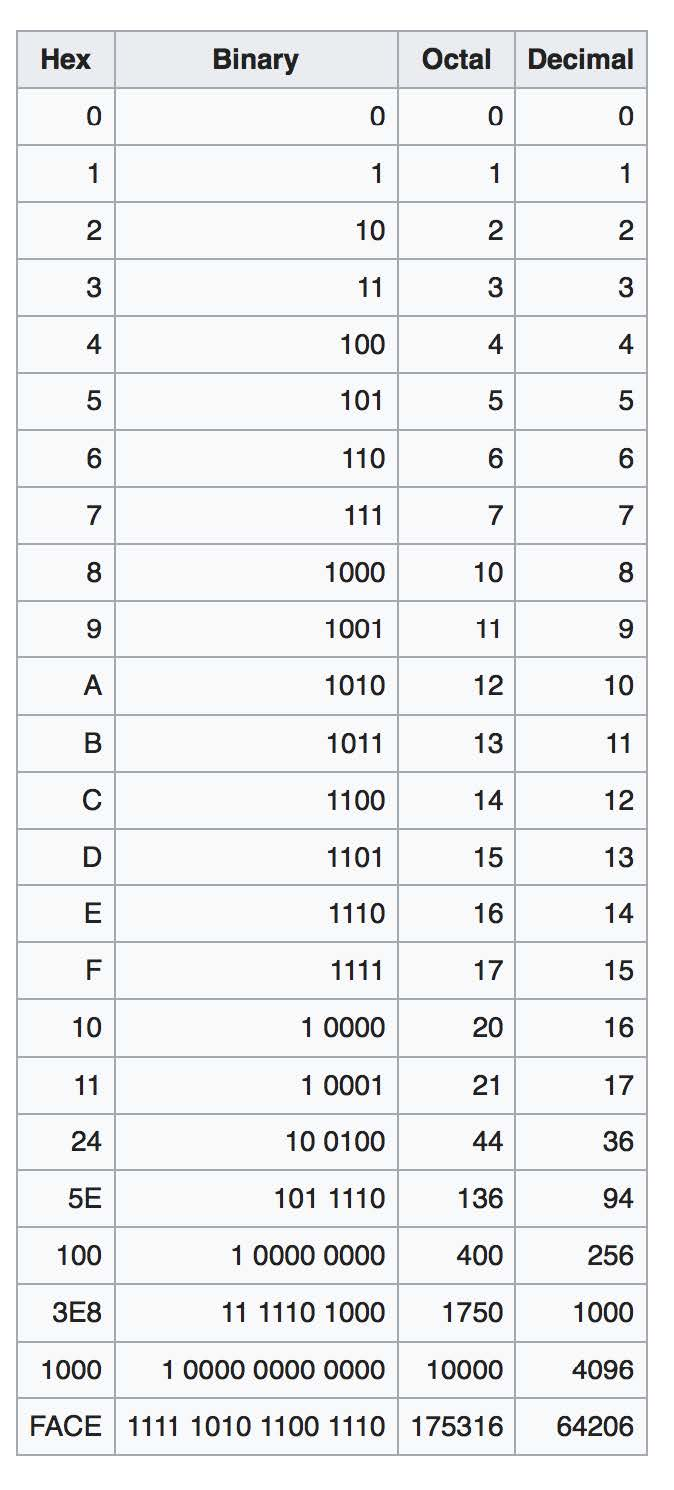
\includegraphics[width = 7cm]{Conversion_table}
\includegraphics[width = 7cm]{Cache_algo}
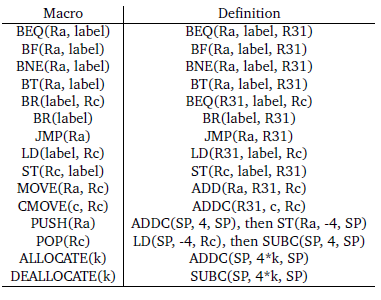
\includegraphics[width = 7cm]{Macro}
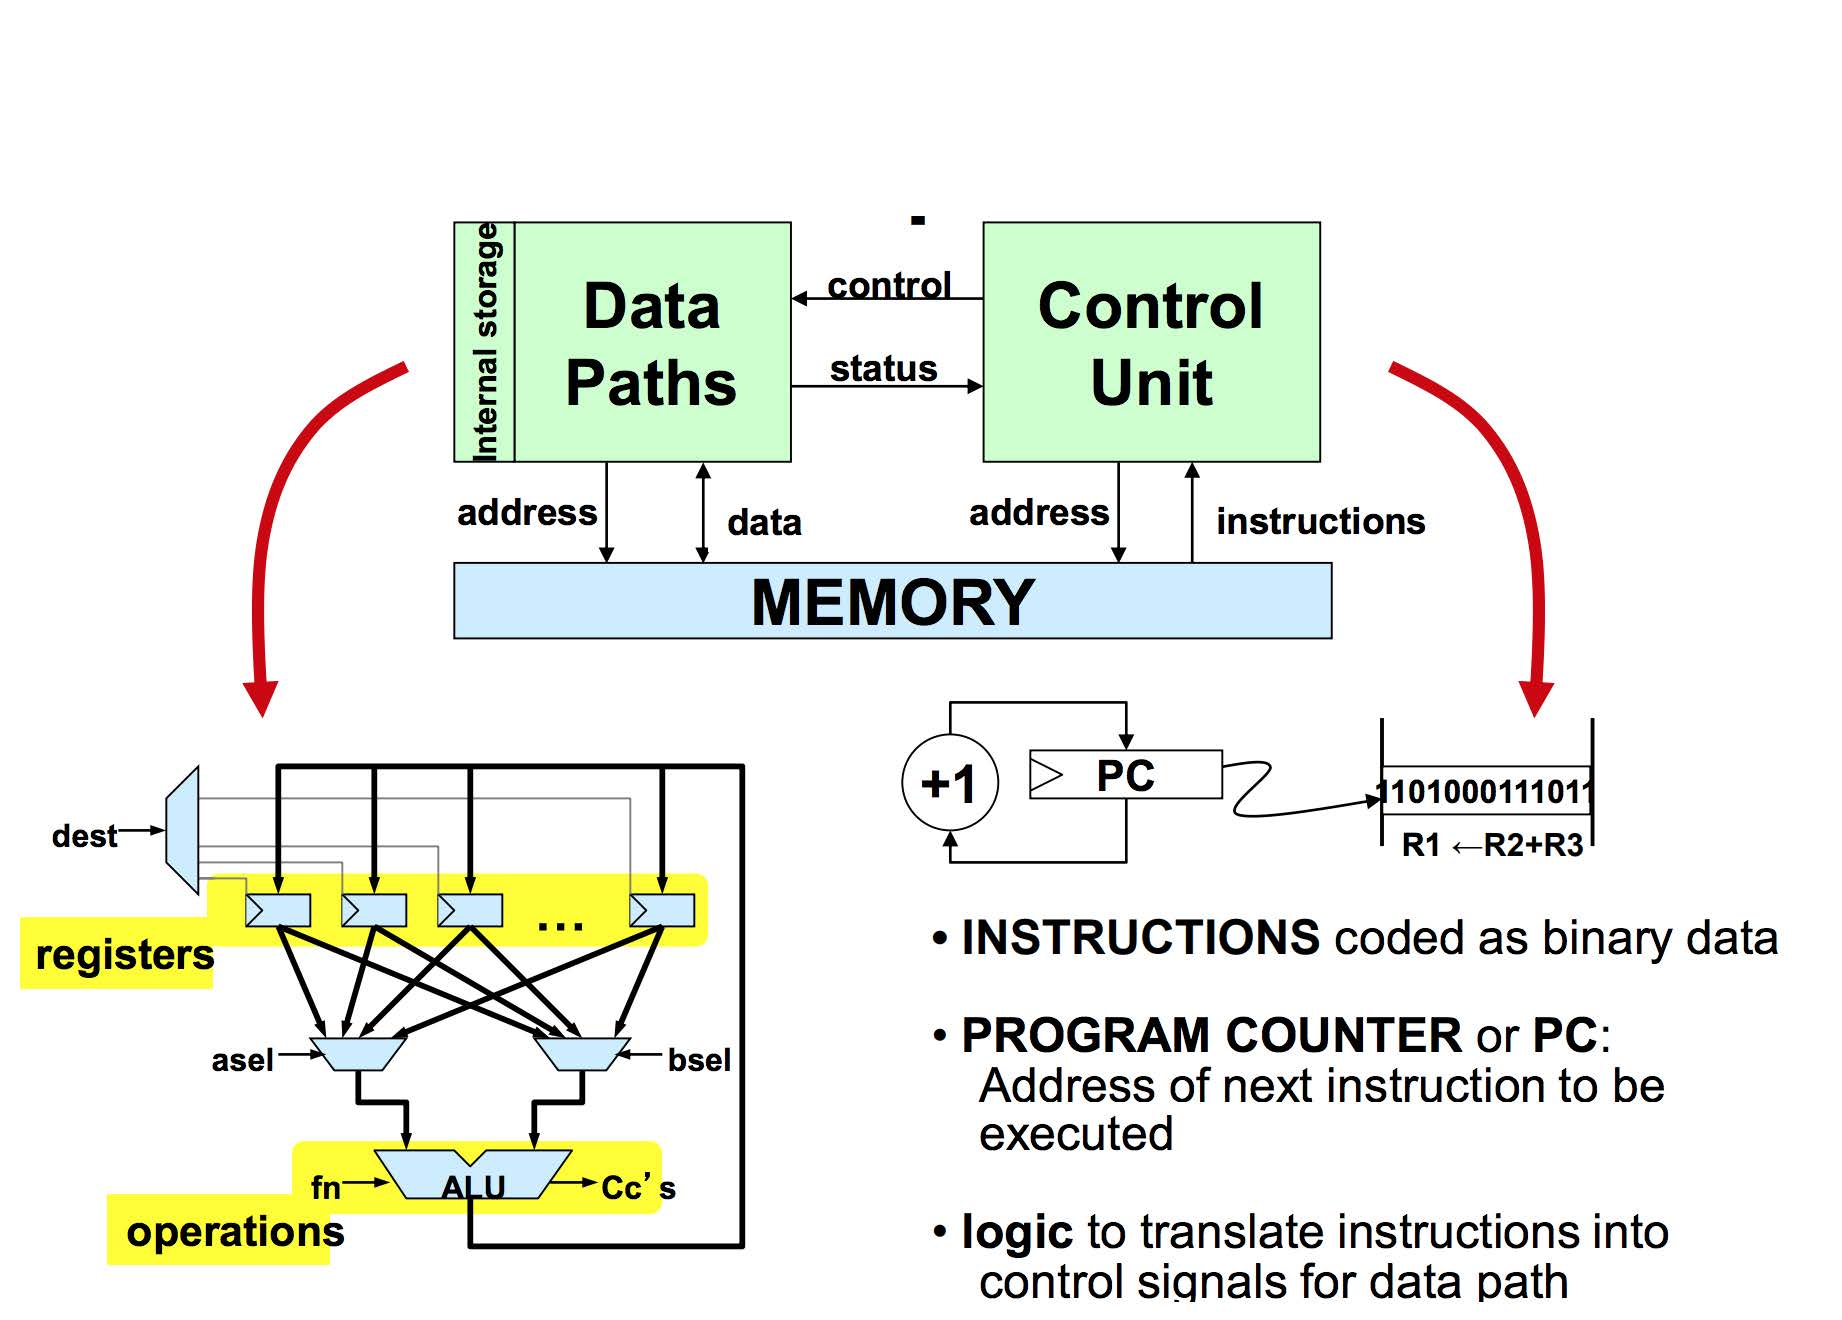
\includegraphics[width = 7cm]{CPU_anatomy}
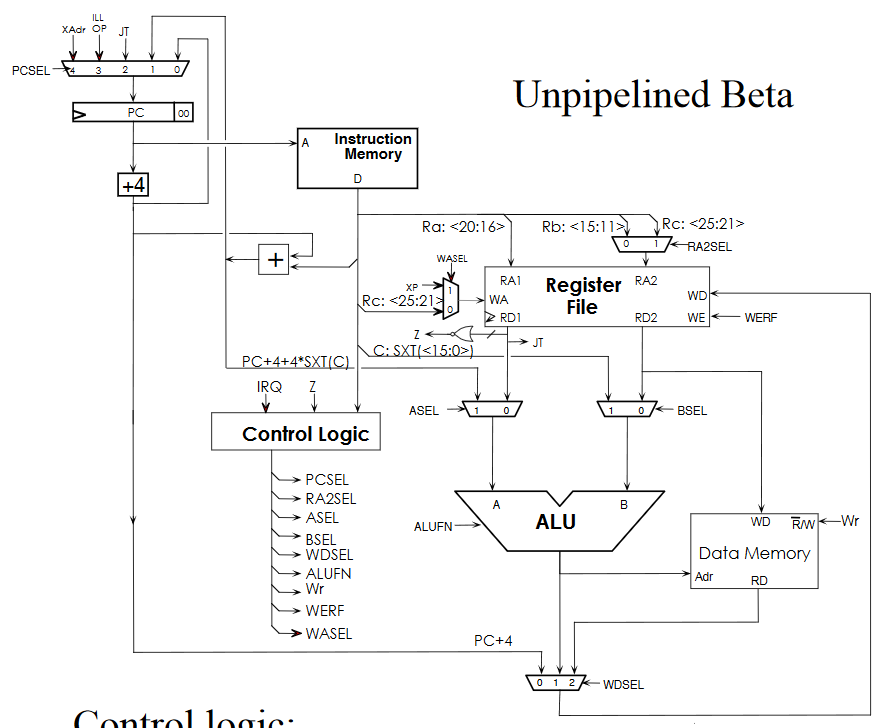
\includegraphics[width = 7cm]{Beta}
\end{multicols*}
\end{document}